% DAFN24 - Robotics - Lecture 1
% Roberto Masocco <roberto.masocco@uniroma2.it>
% May 6, 2024

\documentclass[aspectratio=169]{beamer}

% Slides layout
\usepackage[
    title={Roboticist 101},
    subtitle={Software and middleware for robotics},
    event={DAFN},
    author={Roberto Masocco},
    longauthor={Roberto Masocco},
    email={roberto.masocco@uniroma2.it},
    institute={Tor Vergata},
    longinstitute={University of Rome Tor Vergata},
    department={Department of Civil Engineering and Computer Science Engineering},
    researchgroup={},
    date={May 9, 2024}
]{utvengbeamer}

% Code listings settings
\usepackage[nomath]{lmodern}
\definecolor{codegreen}{rgb}{0 0.5 0}
\definecolor{codered}{rgb}{1 0 0}
\definecolor{codeocher}{rgb}{0.8 0.47 0.13}
\usepackage{listings}
\lstdefinestyle{beamer}{
    basicstyle=\ttfamily\small,
    commentstyle=\color{codegreen},
    breakatwhitespace=false,
    captionpos=b,
    frame=lines,
    keepspaces=true,
    keywordstyle=\color{codered}\bfseries,
    numbers=left,
    numbersep=5pt,
    numberstyle=\footnotesize,
    showspaces=false,
    showstringspaces=false,
    showtabs=false,
    stringstyle=\color{codeocher},
    tabsize=2
}
\lstset{style=beamer}
\lstdefinelanguage{Dockerfile}{
  alsoletter={[, ], _, /},
  morecomment=[l][\color{codegreen}]{\#},
  morekeywords={FROM, RUN, ADD, COPY, LABEL, ENV, ARG, CMD}
}
\lstdefinelanguage{compose}{
  alsoletter={:, -, /},
  morecomment=[l][\color{codegreen}]{\#},
  morekeywords={services:, build:, context:, network_mode:, args:, environment:, command:, volumes:, image:, -}
}

\usepackage{hyperref}
\usepackage{wasysym}

\begin{document}

% --- Title page ---
\frame{\titlepage}

% --- Table of contents ---
\begin{frame}
\frametitle{Roadmap}
\tableofcontents
\end{frame}

% --- Section 1 ---
% Section 1 - Introduction
% Roberto Masocco <roberto.masocco@uniroma2.it>
% May 6, 2024

% ### Introduction ###
\section{Introduction}
\graphicspath{{figs/section1/}}

% --- Information ---
\begin{frame}{Information}
	\begin{itemize}
		\item \textbg{Calendar}: from May 17 to June 14, 2023
		\item \textbg{Topics} (both with practical examples):
		      \begin{enumerate}
			      \item Middleware for robotics
			      \item 3D printing basics (with Simone Mattogno)
		      \end{enumerate}
		\item \textbg{Materials} (for my part):
		      \begin{itemize}
			      \item Code repository: \href{https://github.com/IntelligentSystemsLabUTV/ros2-examples}{\color{blue}\underline{github.com/ros2-examples}} (\texttt{humble} branch)
			      \item Lectures: \href{https://github.com/stars/robmasocco/lists/lectures}{\color{blue}\underline{github.com/robmasocco}}, Teams directory (this lecture is \href{https://github.com/robmasocco/DAFN23_Robotics_1}{\color{blue}\underline{here}})
		      \end{itemize}
		\item \textbg{Useful background} (for my part):
		      \begin{itemize}
			      \item Basics of C and Python programming
			      \item Basics of Git workflow (check out \href{https://www.atlassian.com/git/tutorials/what-is-git}{\color{blue}\underline{this tutorial}} by Atlassian)
			      \item Everyday Linux commands and a Unix-like system
		      \end{itemize}
		      \visible<2>{
		\item \textbg{Exam}: ... ask Prof. Carnevale \smiley
		      }
	\end{itemize}
\end{frame}

% --- Program ---
\begin{frame}{Program}{Middleware for robotics}
	\begin{enumerate}
		\item Roboticist 101 - Software and middleware for robotics
		\item ROS 2 - Workflow and basic communication
		\item ROS 2 - Advanced communication
		\item ROS 2 - Node configuration
		\item ROS 2 - Sensor sampling and image processing
		\item ROS 2 - Interfacing with the data space
		\item microROS - Bridging the gap
	\end{enumerate}
\end{frame}

% --- The roboticist ---
\begin{frame}{The roboticist}{A new path for control engineers}
	\begin{columns}
		\column{.5\textwidth}
		A \textbg{control engineer} is a specialist in the \textbg{design} of controllers to drive \textbg{dynamic systems}; the implementation was traditionally left to other specialists.\\
		A \textbg{roboticist} is a specialist capable of designing, \textbg{building}, and \textbg{programming} complex \textbg{autonomous systems}; with skills ranging from computer science to other disciplines.
		\begin{block}{}
			\centering
			\textbf{A control engineer can be very effective as a roboticist.}
		\end{block}

		\column{.5\textwidth}
		\begin{figure}
			\centering
			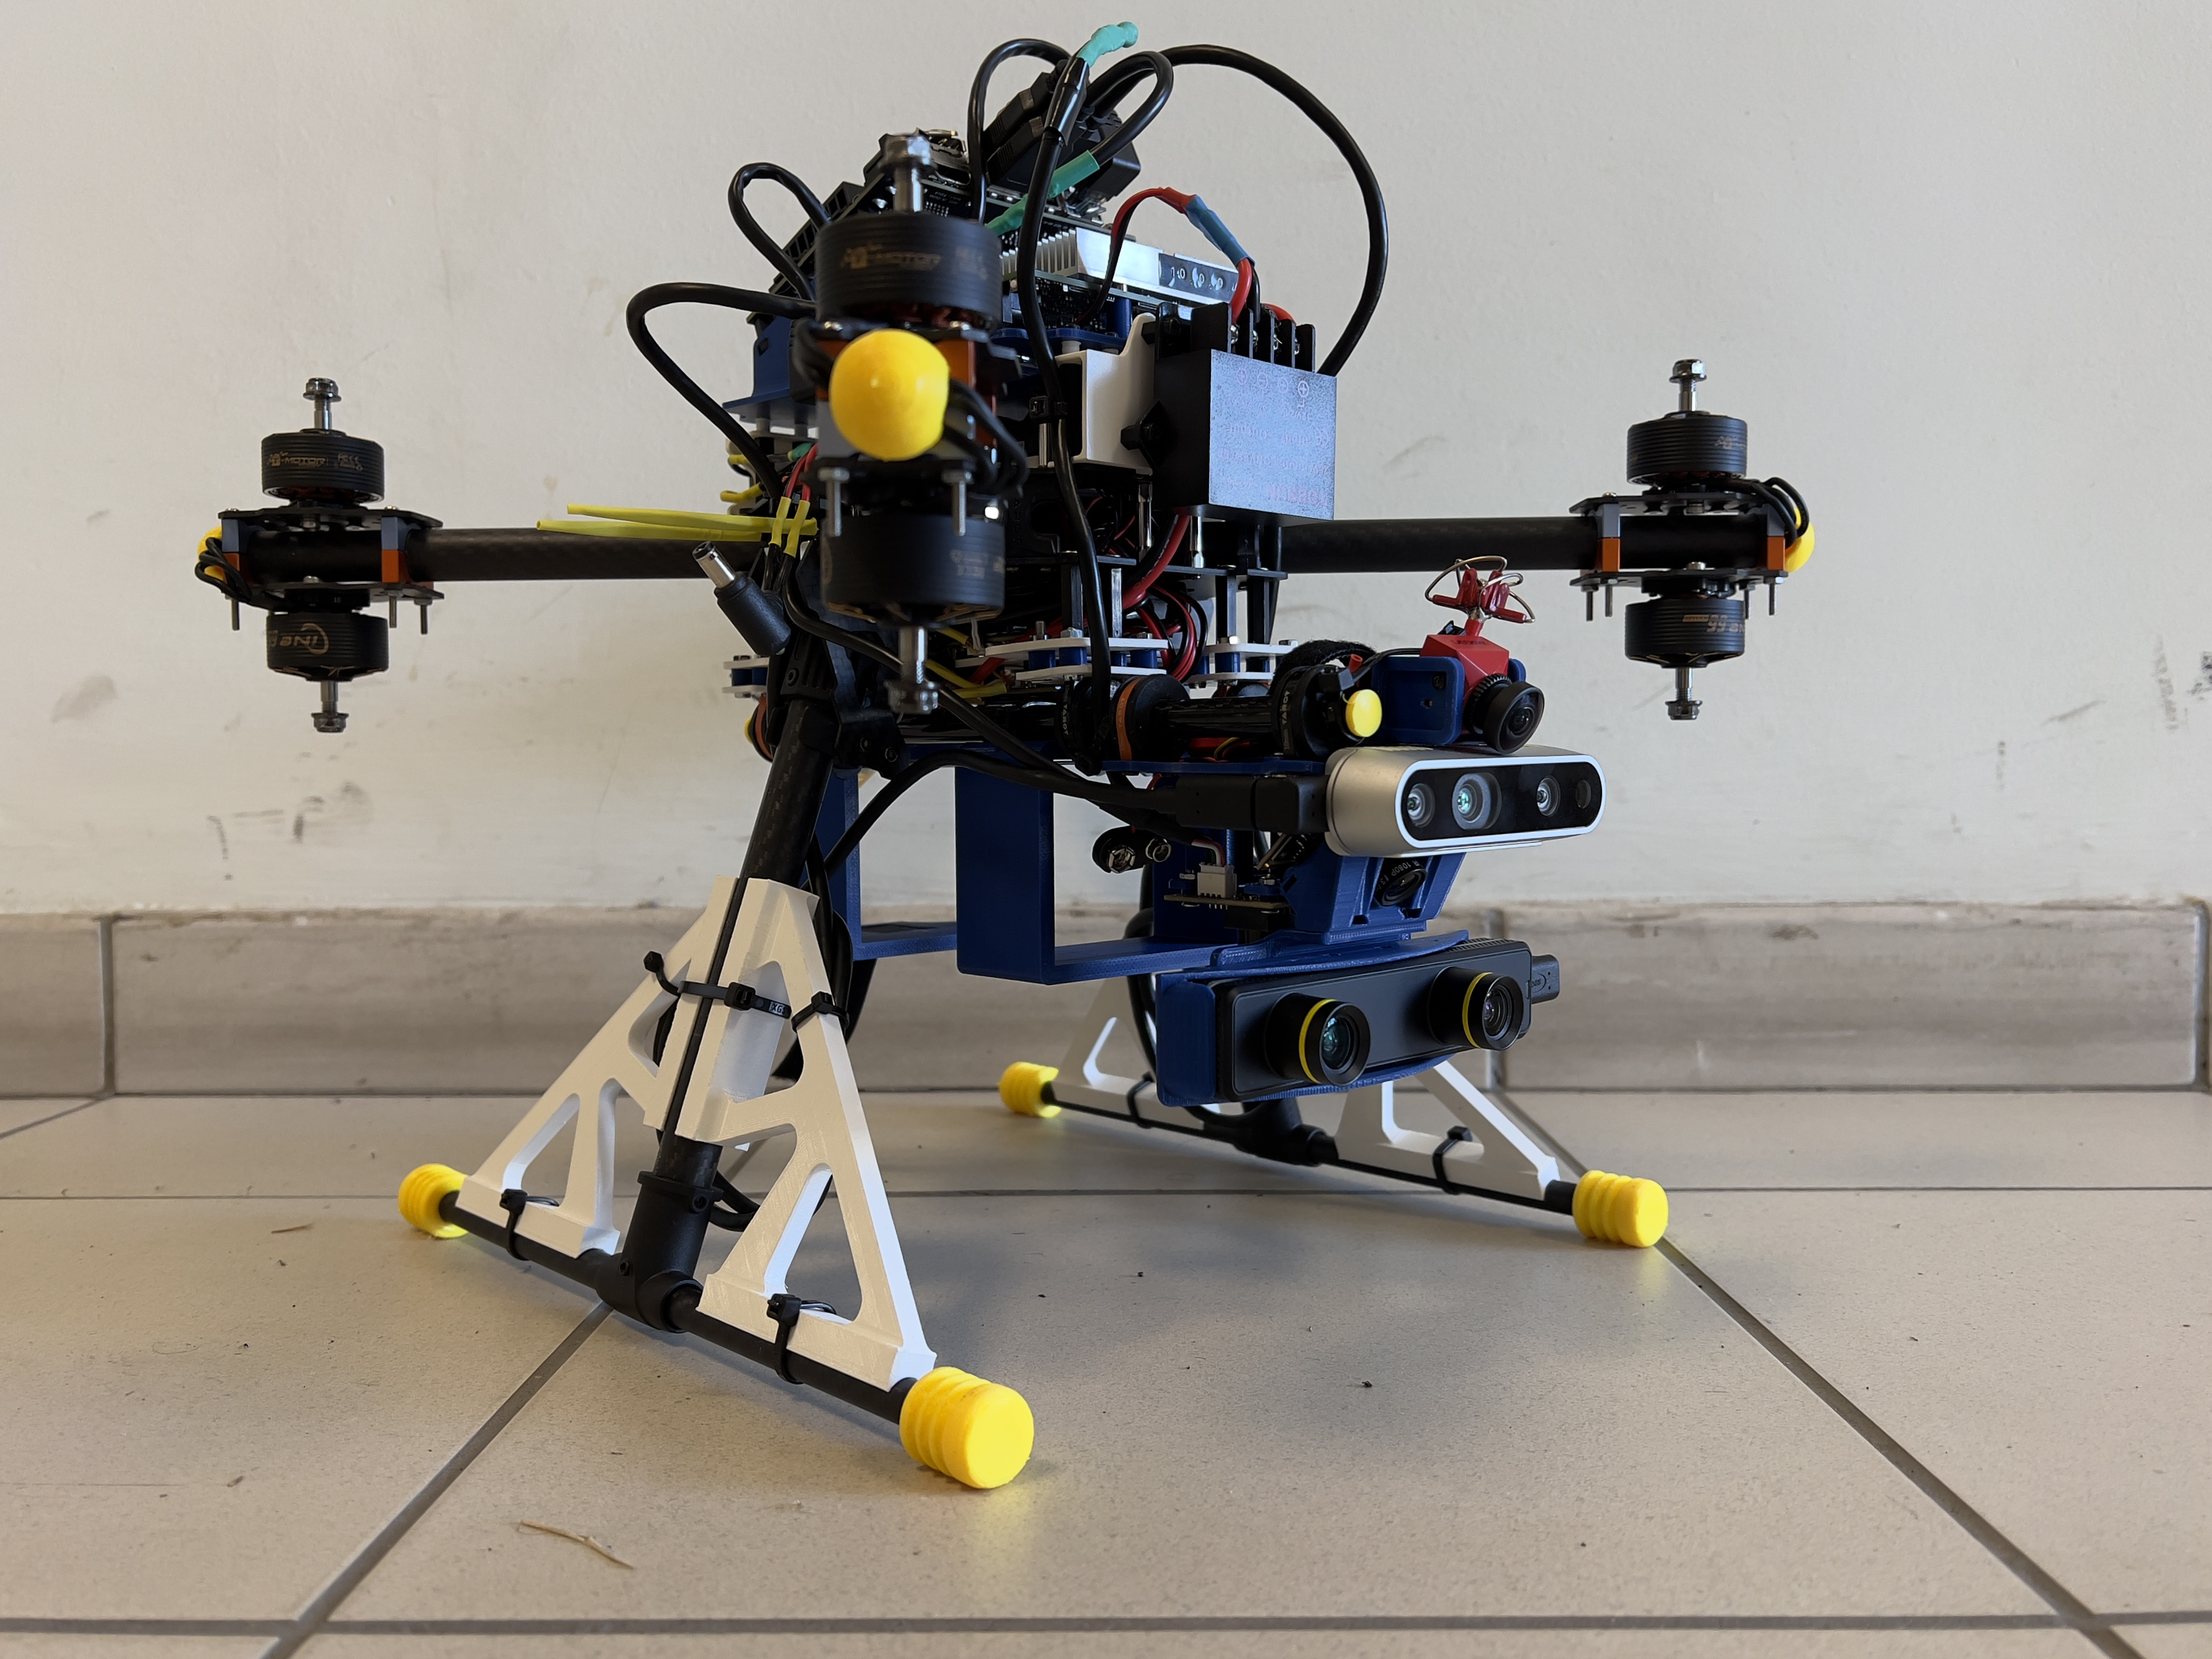
\includegraphics[width=.8\textwidth]{stanis}
			\caption{Stanis autonomous drone prototype.}
			\label{fig:stanis}
		\end{figure}
	\end{columns}
\end{frame}
\begin{frame}{The roboticist}{A new path for control engineers}
	\begin{columns}
		\column{.5\textwidth}
		A \textbg{roboticist} can usually:
		\begin{itemize}
			\item \textbg{design} solutions to complex problems;
			\item \textbg{develop} parts of a robot, or entire \textbg{control architectures};
			\item \textbg{deploy} and test software and hardware solutions;
			\item make use of modern \textbg{hardware accelerators} and robotics-oriented hardware.
		\end{itemize}
		Industries are looking for roboticist for their \textbg{versatile skill set}.

		\column{.5\textwidth}
		\begin{figure}
			\centering
			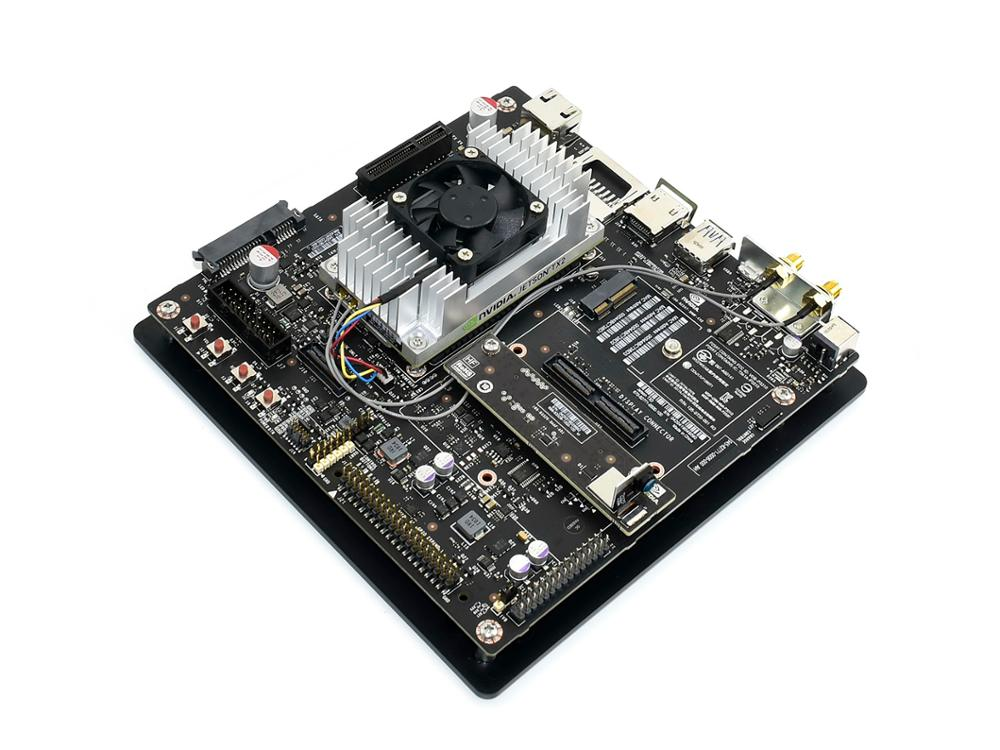
\includegraphics[width=.9\textwidth]{tx2}
			\caption{Nvidia Jetson TX2 developer kit.}
			\label{fig:tx2}
		\end{figure}
	\end{columns}
\end{frame}


% --- Section 2 ---
% Section 2 - Middleware in robotics
% Roberto Masocco <roberto.masocco@uniroma2.it>
% May 14, 2023

% ### Middleware in robotics ###
\section{Middleware in robotics}
\graphicspath{{figs/section2/}}

% --- What is middleware? ---
\begin{frame}{What is middleware?}
	\begin{figure}
		\centering
		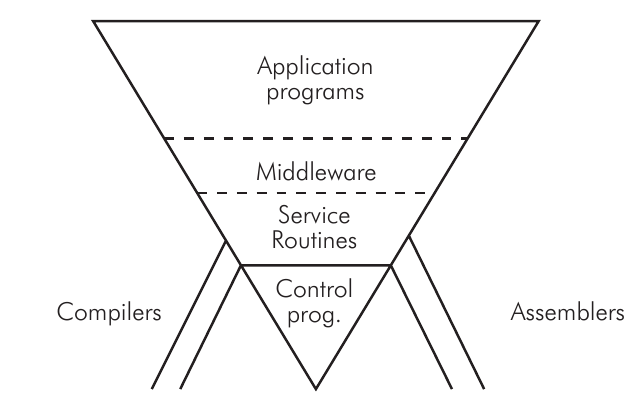
\includegraphics[width=.64\textwidth]{softwarePyramid.png}
		\caption{Software organization in a general-purpose computer system.}
		\label{fig:swpyramid}
	\end{figure}
\end{frame}
\begin{frame}{What is middleware?}
	\begin{block}{Definition of middleware}
		\justifying
		The term \textbf{middleware} identifies a kind of software that offers common services and functionalities to applications in addition to what an operating system usually does.
	\end{block}
	\justifying
	Middlewares are usually implemented as \textbg{libraries} that application programmers can use via appropriate \textbg{APIs}.
\end{frame}

% --- Middleware in robotics ---
\begin{frame}{Middleware in robotics}
	\justifying
	New problems arising when developing software for modern autonomous systems:
	\begin{itemize}
		\item integration of \textbg{sophisticated hardware} (microcontrollers, hardware accelerators, SBCs);
		\item \textbg{software} organization and maintenance;
		\item \textbg{communication} (involves both hardware and software!);
		\item debugging and \textbg{testing}.
	\end{itemize}
	\begin{block}{}
		\centering
		Middlewares can help to tackle and solve each one!
	\end{block}
\end{frame}

% --- Data Distribution Service ---
\begin{frame}{Data Distribution Service}
	\begin{block}{Definition of DDS}
		A DDS is a \textbf{publish-subscribe middleware} that handles communications between \textbf{real-time} systems and software over the network.
	\end{block}
	DDSs are currently used in automotive, aerospace, military...\\
	Their implementations follow an \textbg{open standard} that defines:
	\begin{itemize}
		\item \textbg{serialization} and \textbg{deserialization} of data packets (\texttt{RTPS Wire Protocol});
		\item \textbg{security protocols} and cryptographic operations;
		\item enforcing of \textbg{Quality of Service} policies to organize transmissions (specifying things like \textbg{queue sizes}, \textbg{best-effort} or \textbg{reliable} transmissions...);
	\end{itemize}
\end{frame}
\begin{frame}{Data Distribution Service}
	\begin{itemize}
		\item automatic discovery of \textbg{DDS participants} (over \textbg{multicast-IP/UDP}) and transmission of data (over \textbg{unicast-IP/UDP}) (\texttt{Discovery Protocol}).
	\end{itemize}
	\begin{figure}
		\centering
		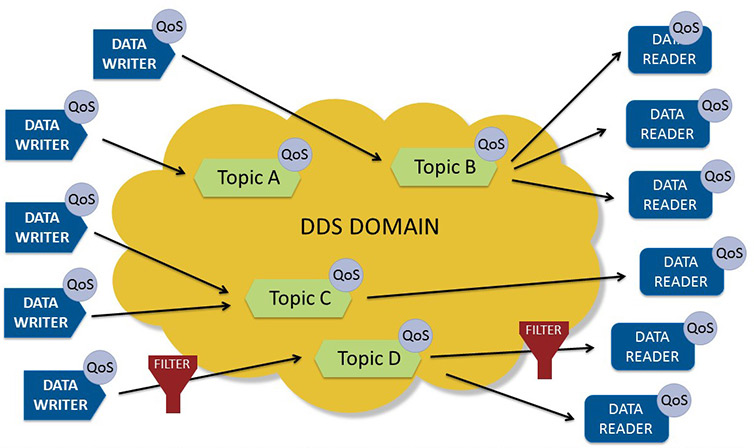
\includegraphics[scale=.32]{ddsDomain.jpg}
		\caption{Scheme of a DDS-based network (data space).}
		\label{fig:ddsdomain}
	\end{figure}
\end{frame}
\begin{frame}{Data Distribution Service}
	DDS participants can either \textbg{publish to} or \textbg{subscribe to} a \textbg{topic}.
	\begin{block}{Definition of DDS topic}
		A DDS topic is \textbf{uniquely identified} by three attributes:
		\begin{itemize}
			\item a \textbf{name}, \emph{i.e.}, a human-readable character string;
			\item an \textbf{interface}, \emph{i.e.}, a custom packet format that specifies what data is carried over it (\emph{e.g.}, strings, numbers, arrays...);
			\item a \textbf{QoS policy} that specifies how transmissions should be performed.
		\end{itemize}
	\end{block}
	\begin{block}{}
		\centering
		\textbf{Changing even only one of the above results in a completely different topic!}
	\end{block}
\end{frame}


% --- Section 3 ---
% Section 3 - ROS 2 overview
% Roberto Masocco <roberto.masocco@uniroma2.it>
% May 6, 2024

% ### ROS 2 overview ###
\section{ROS 2 overview}
\graphicspath{{figs/section3/}}

% --- What is ROS 2? ---
\begin{frame}{What is ROS 2?}
	\begin{columns}
		\column{.5\textwidth}
		\only<1>{
			\nolistindent ROS 2 is a \textbg{DDS-based}, \textbg{open-source} middleware for robotic applications.\\
			It allows developers to build and manage \textbg{distributed control architectures} made of many modules, usually referred to as \textbg{nodes}.
		}
		\only<2>{
			\nolistindent \nolistindent ROS 2 currently supports \textbg{C++} and \textbg{Python} for application programming, and runs natively on \textbg{Ubuntu Linux 22.04}.
			\newline\newline
			New versions are periodically released as \textbg{distributions}: the current LTS one is \textbg{Humble Hawksbill}; the development version is \textbg{Rolling Ridley} and can only be compiled from source.\\
			It is available as \textbg{binary \texttt{deb} packages} for \texttt{x86} and \texttt{ARMv8} architectures.
			\newline\newline
			A \textbg{distribution} is a collection of software packages: \textbg{libraries}, \textbg{tools}, and \textbg{applications}.
		}

		\column{.5\textwidth}
		\begin{figure}
			\centering
			
\includegraphics[width=.8\textwidth]{ros2Logo.jpg}
			\caption{ROS 2 logo.}
			\label{fig:ros2logos}
		\end{figure}
	\end{columns}
\end{frame}

% --- Why ROS 2? ---
\begin{frame}{Why ROS 2?}
	\begin{columns}
		\column{.5\textwidth}
		The ROS project started in 2007, to provide a middleware that could solve the \textbg{software integration} and \textbg{communication} problems in robotics. It has evolved much since then.
		\newline\newline
		ROS 2 helps to design and build \textbg{distributed control architectures}, providing a common ground for the \textbg{integration} of different systems, sensors, actuators, and algorithms.\\
		It is a common framework for the development of \textbg{robotics software}.
		\newline\newline
		Its adoption is still limited because of familiarity with the original ROS, but it is \textbg{growing}.

		\column{.5\textwidth}
		\begin{figure}
			\centering
			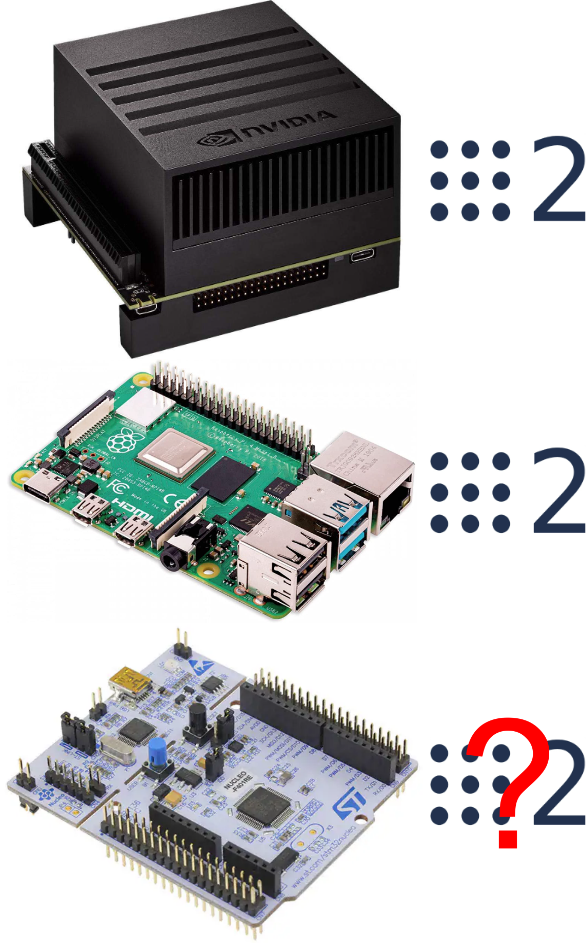
\includegraphics[scale=.17]{why_ros2.png}
			\label{fig:whyros2}
			\caption{STM32 (bottom), Raspberry Pi (middle), and Nvidia Xavier AGX (top).}
		\end{figure}
	\end{columns}
\end{frame}

% --- Main Features ---
\begin{frame}{Main features}
	As a middleware, it offers many \textbg{services to roboticists}, including:
	\begin{itemize}
		\item \textbg{three communication paradigms}, easy to set up and based on the DDS: \textbg{messages}, \textbg{services} and \textbg{actions};
		\item organization of software packages, allowing for \textbg{redistribution and code reuse}, thanks to the \textbg{\texttt{colcon}} package manager;
		\item module configuration tools: \textbg{node parameters} and \textbg{launch files};
		\item integrated \textbg{logging subsystem} (involves both console and log files);
		\item CLI \textbg{introspection tools} for debugging and testing;
	\end{itemize}
\end{frame}
\begin{frame}{Main features}
	\begin{itemize}
		\item may be integrated in some \textbg{simulators} (\emph{e.g.}, Gazebo) and \textbg{visualizers} (\emph{e.g.}, RViz).
	\end{itemize}
	\begin{figure}
		\centering
		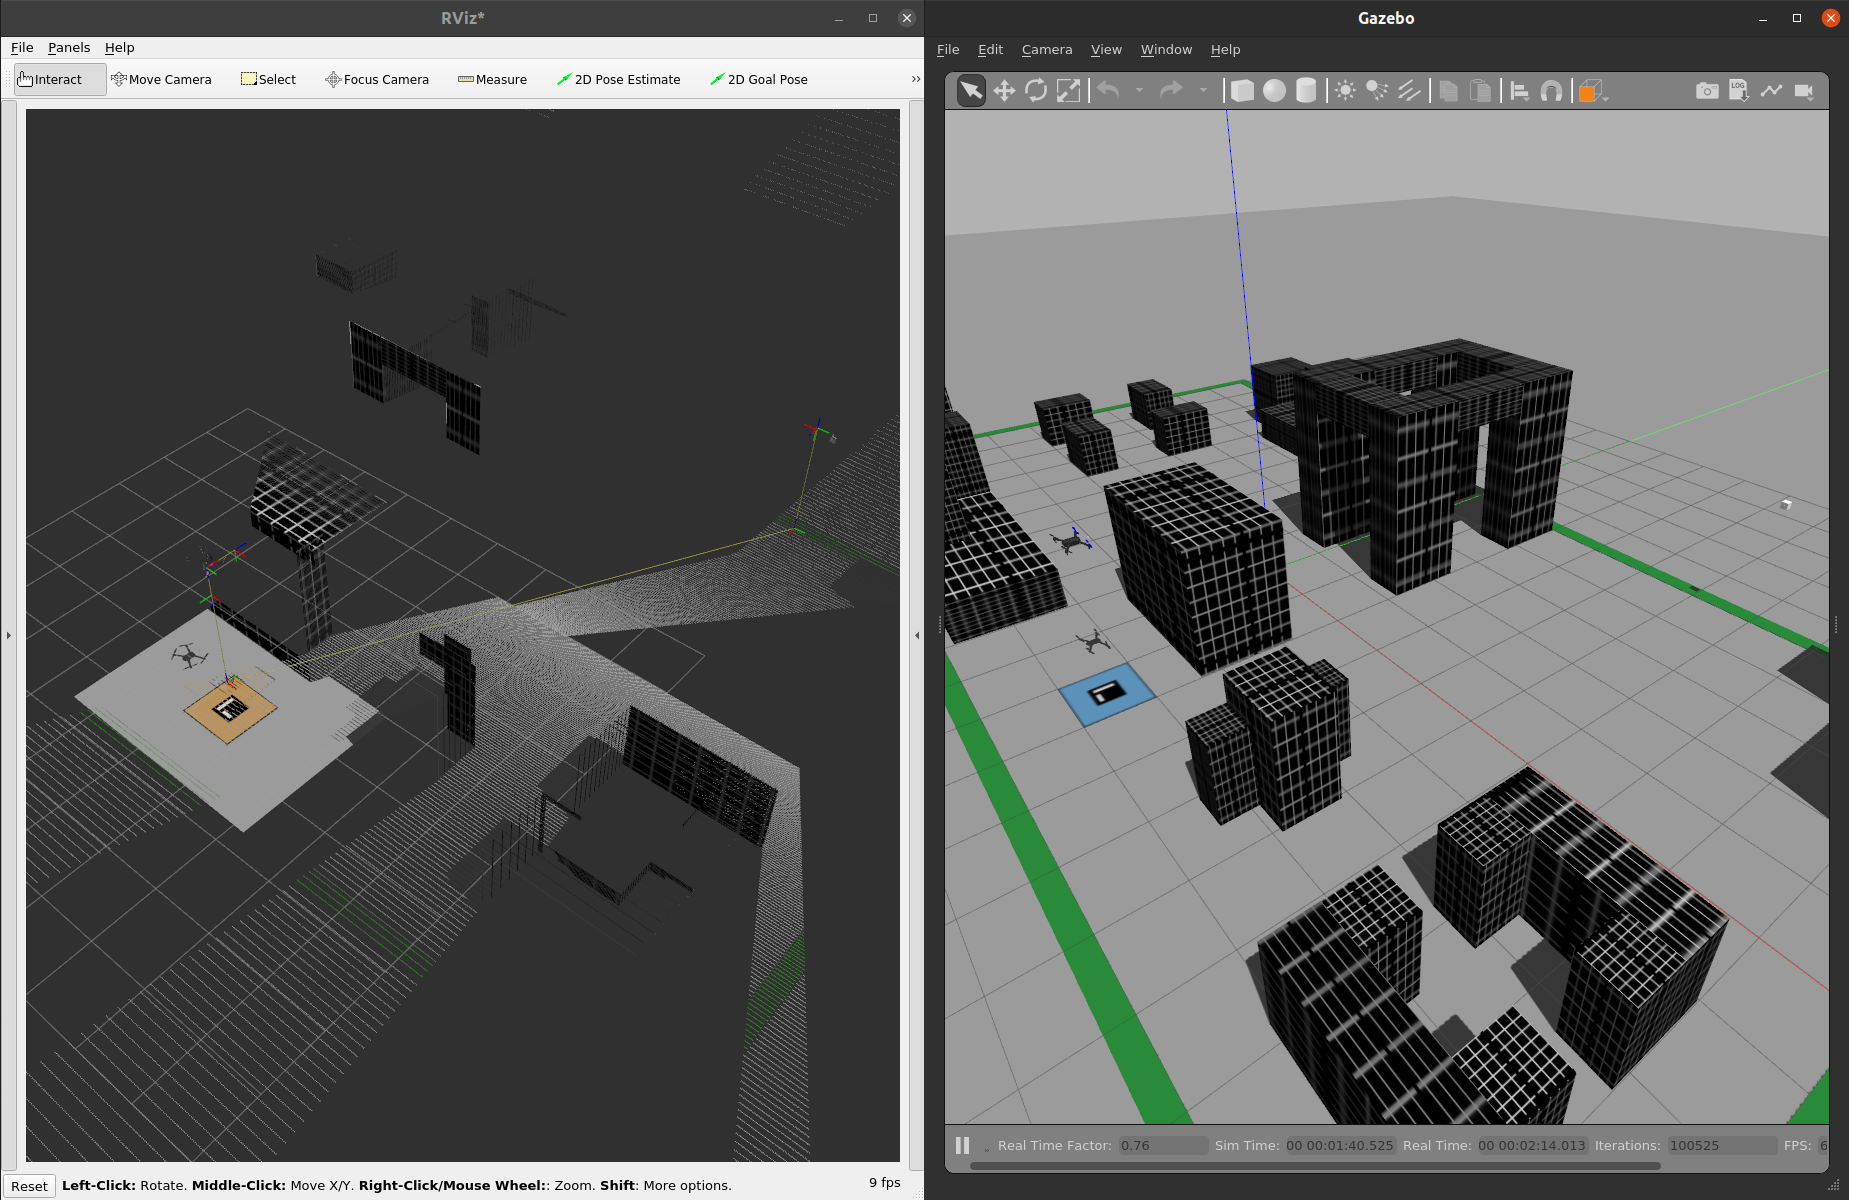
\includegraphics[scale=.133]{simulation.png}
		\label{fig:sim}
		\caption{Simulated drone in Gazebo Classic and RViz.}
	\end{figure}
\end{frame}

% --- Application Programming Interface ---
\begin{frame}{Application Programming Interface}{Deep dive into ROS 2 internals}
	A \textbg{ROS 2 installation}, from bottom to top, works as follows:
	\begin{enumerate}
		\item \textbg{DDS}: the middleware that implements the \textbg{communication layer} (many different implementations are supported).
		\item \textbg{RMW}: ROS MiddleWare, is the \textbg{DDS abstraction layer}, which allows to use different DDS implementations without changing the application code.
		\item \textbg{rcl}: ROS Client Support Library (C), implements basic entities: \textbg{nodes}, \textbg{publishers}, \textbg{subscribers}, \textbg{services}, \textbg{clients}, and \textbg{timers}.
		\item \textbg{rclc}/\textbg{rclcpp}/\textbg{rclpy}: ROS Client Library (C/C++/Python), implements the same entities as \texttt{rcl}, plus extended functionalities like the \textbg{executor}: a job scheduler.
	\end{enumerate}
	Then, there are \textbg{packages}: libraries, tools, and applications, both officially provided and community-contributed. The entire ROS 2 codebase is on \href{https://github.com/ros2}{\color{blue}\underline{GitHub}}.\\
  Keep this in mind during debugging, or while looking for information on an API!
\end{frame}
\begin{frame}{Application Programming Interface}{How a ROS 2 application works}
	The most important entity is the \textbg{node}, whose functionalities are specified upon creation.\\
	A node must usually do \textbg{a single thing}, being the \textbg{unit} in a \textbg{distributed architecture}.\\
	With its class methods, it can:
	\begin{itemize}
		\item act as an \textbg{entry point} towards the DDS layer, to handle communications;
		\item embed \textbg{software modules} like data, algorithms, and threads, that implement the application logic;
		\item register \textbg{callbacks} to handle \textbg{events}, such as timers or incoming messages.
	\end{itemize}
	Thus, it is both an \textbg{operational unit} and a \textbg{communication endpoint}.\\
	Nodes are usually handled by \textbg{executors}, which are responsible for scheduling and processing their \textbg{ROS-workload}.
	\begin{block}{}
		\centering
		\textbf{Nodes are just objects in your application: they can embed any kind of software module, but they do not limit the design to their paradigms.}
	\end{block}
\end{frame}

% --- Executors: events and callbacks ---
\begin{frame}{Executors}{Handling events and callbacks}
	\begin{figure}
		\centering
		\includesvg[scale=.45]{ROS2_executor_scheme.svg}
		\label{fig:executorscheme}
		\caption{ROS 2 event-based programming paradigm.}
	\end{figure}
\end{frame}
\begin{frame}{Executors}{Handling events and callbacks}
	\begin{enumerate}
		\item Middleware functionalities trigger \textbg{(a)synchronous events}.
		\item Events are handled by \textbg{background jobs}, coded in \textbg{callbacks} by the programmer.
		\item Callbacks are \textbg{registered} into a \textbg{node} when its functionalities are specified (\emph{e.g.}, upon creation).
		\item The workload that a node carries is scheduled and processed by an \textbg{executor}, single- or multi-threaded.
	\end{enumerate}
	\begin{alertblock}{}
		\centering
		Executors implement a \textbr{round-robin}, \textbr{non-preemptive} policy that \textbr{always prioritizes timers}.
	\end{alertblock}
\end{frame}

% --- Flaws ---
\begin{frame}{Flaws}
	\visible<1->{
		\begin{alertblock}{ROS 2 biggest flaws (as of today)}
			The main concerns arise when developing low-level stuff:
			\begin{itemize}
				\item \textbr{the DDS layer is almost completely abstracted}, so non-standard network configurations may get tricky;
				\item the internal job scheduling algorithm (namely the \textbr{executor}) is \textbr{not suited for hard real-time applications} because of its \textbr{non-preemptive} nature.
			\end{itemize}
		\end{alertblock}
	}
	\visible<2>{
		What to do when development gets to a really low level?
		\begin{itemize}
			\item Hand off stuff to dedicated \textbg{microcontrollers}.
			\item Use \textbg{micro-ROS}: hard real-time ROS 2 on microcontrollers and different communication interfaces.
		\end{itemize}
	}
\end{frame}


\end{document}
